\chapter{Evaluation}\label{chap:evaluation}
In this chapter, we introduce the provided datasets we evaluate the models on.
We then set hypotheses about the assumed performances of the chosen models on
our datasets. Next, we describe our process of training. We briefly mention the
technologies we have used and how we have chosen our models' parameters.
Finally, we present our achieved results and discuss them.

\section{Datasets}
We are provided with three datasets by the company SANEZOO EUROPE.
Unfortunately, two of the datasets cannot be published as they are protected
under a confidentiality agreement. However, we provide sufficient
characteristics of the datasets. We summarize the basic information of the
datasets in Table \ref{tab:datasets}. Detailed description is provided below
the table.

\begin{table}[h]
	\centering
	\begin{tabular}{|l|l|l|l|l|}
		\hline
		\bld{Type}       & \bld{Difficulty} & \bld{Size} & \bld{Classes} & \bld{Publishable} \\ \hline
		Candies          & Easy             & 150        & 1             & Yes               \\
		Metal parts      & Medium           & 8272       & 7             & No                \\
		Medical supplies & Hard             & 805        & 11            & No                \\ \hline
	\end{tabular}
	\caption{Datasets summary.}
	\label{tab:datasets}
\end{table}


\begin{figure}[H]

	\begin{subfigure}[c]{0.5\textwidth}
		\centering
		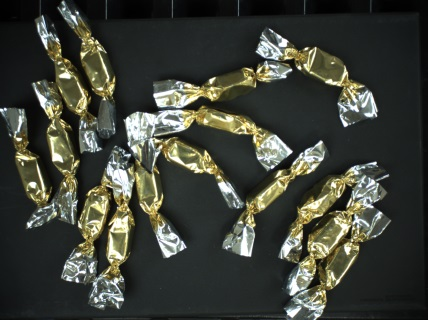
\includegraphics[width=0.9\linewidth]{Sources/Figures/sparse.jpg}
		\caption{Sparse example}

	\end{subfigure}
	\begin{subfigure}[c]{0.5\textwidth}
		\centering
		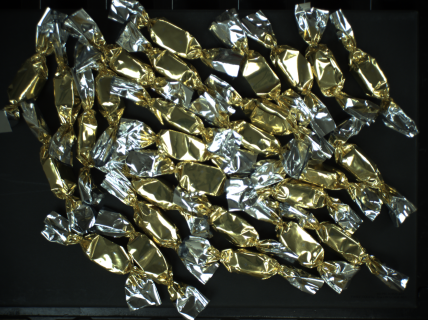
\includegraphics[width=0.9\linewidth]{Sources/Figures/dense.png}
		\caption{Dense example}

	\end{subfigure}

	\caption{Examples of candies dataset.}
	\label{fig:candies}
\end{figure}

\subsection*{Candies dataset}
Only the first dataset is publishable; thus, we provide a
visual example image in Figure \ref{fig:candies}. The images consist only of a
single class -- a golden candy. The density of objects (how densely they cover
the image) varies through the dataset (see Figure \ref{fig:candies}). Object
occlusions can occur in dense images; therefore, the dataset is not trivial.
However, compared to our other datasets, it is still a simpler dataset as it
strictly contains only a single class without foreign objects. Therefore, we
assign an easy difficulty to this dataset.

\subsection*{Metal parts dataset}
The second dataset consists of images with small
metal parts (such as shafts, rings, casings). See Figure \ref{fig:parts} for
rough illustration. The objects are placed in a plastic bin. There is always
only one class of objects on a single image. The images are taken from a
top-down perspective, similarly as in Figure \ref{fig:candies}. However, they
are taken from various angles. The density of objects also differ through the
dataset as in the first dataset (you can imagine a pile of metal parts).

\begin{figure}[ht]
	\centering
	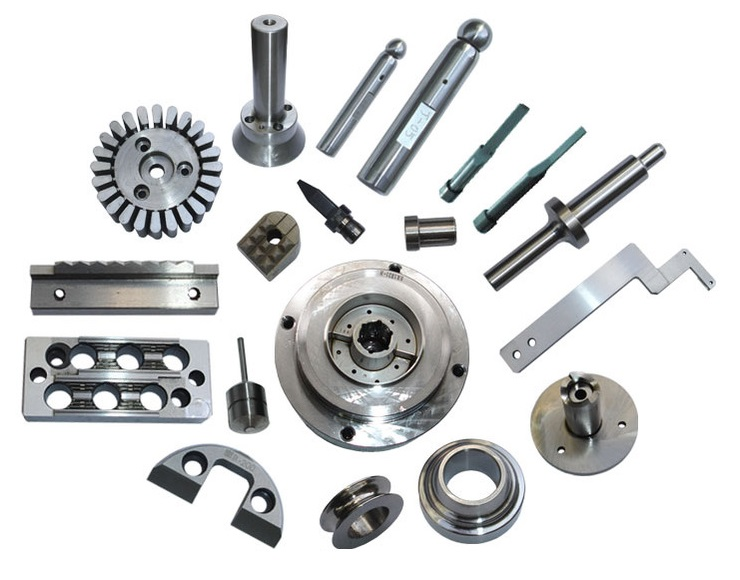
\includegraphics[height=0.35\linewidth]{Sources/Figures/metal_parts.jpg}
	\caption{An illustration of classes from metal parts dataset. Taken from
		\cite{parts}.}
	\label{fig:parts}
\end{figure}

\subsection*{Medical supplies dataset}
The last set is made up of sequences of images
taken from an assembly line's top view. The images capture a manual assembly of
packages that are consisted of medical items (such as bandages, plastic cups, or
surgery tools). We assign a hard difficulty to this dataset because of the
non-static environment. To be more specific, the packages are in motion in some
images; therefore, the objects are slightly blurred. Moreover, occlusion of
objects occurs in the image very often since the operator does the packing
manually, and the objects are stacked on top of each other. Some objects are
tough to distinguish if they are next to each other (imagine a pile of cotton
balls). The images are taken from above the operator similarly as in the first
dataset.

\section{Hypotheses}
\label{sec:hypotheses}
Let us recapitulate the models we evaluate:
\begin{itemize}
	\item Faster R-CNN with ResNet-50 backbone without FPN,
	\item Cascade R-CNN with ResNet-50 backbone with FPN,
	\item RetinaNet with ResNet-50 backbone with FPN.
\end{itemize}
We set hypotheses based on the results obtained in the models' original papers
\cite{fasterrcnn,cascadercnn,retinanet} and the \bld{Detectron2's} benchmark
results \cite{detectron}.

\renewcommand{\theenumi}{\alph{enumi}}
\begin{enumerate}
	\item Models will perform better on average on our datasets than on COCO
	      datasets \cite{coco} by a significant margin as the COCO dataset is
	      very hard.
	\item Faster R-CNN serves as a baseline and will perform the worst. Cascade
	      R-CNN should perform better than RetinaNet R-50.
	\item RetinaNet R-50 should have the fastest inference speed per image.
	\item All models should achieve at least 1–2 \bld{FPS (frames per second)}
	      speed.
\end{enumerate}

The (d) hypotheses is a minimal \bld{industrial requirement} for the models.
Models that are slower than 1 FPS are not very useful. We need different FPS for
different use cases. For example, a lower FPS would be sufficient for a
surface inspection. On contrary, the camera systems of autonomous vehicles
demand much higher FPS.

\section{Training}
The models were evaluated by \bld{Detectron2} object detection framework
\cite{detectron} based on Python deep learning library \bld{PyTorch}
\cite{pytorch}. Detectron2 includes various pretrained object detection
models and tools for creating, training and evaluating of the models. We have
modified the framework's \texttt{DefaultTrainer} class to meet our needs. We
list some of the modifications below:
\begin{itemize}
	\item The \texttt{DefaultTrainer} trains the model for a given number of
	      iterations (one training step of a minibatch). However, it is more
	      common to set the training for a given number of \bld{epochs}. One
	      epoch corresponds to one pass of the full training set of data. Thus,
	      the number of iterations of one epoch corresponds to fraction of the
	      training set's size to minibatch size. We have implemented this
	      simple conversion.
	\item The interval of a periodical output and periodical saving of weights
	      (\bld{checkpoint}) of the training process was fixed. We have modified
	      the behavior to output the intermediate results after an arbitrary
	      number of iterations.
	\item By default, the training process does not show the validation loss in
	      every checkpoint output. Therefore, we have implemented a
	      \texttt{ValidationLoss} hook class that computes the validation loss
	      after every checkpoint's training step.
\end{itemize}
To train a model with Detectron2, we had to convert our datasets' annotations to
Detectron2's standard format.\footnote{
	\url{https://detectron2.readthedocs.io/tutorials/datasets.html
		\#standard-dataset-dicts}
}
The format is a list of Python dictionaries. Each dictionary describes each
image and the objects included in the image. We have converted the datasets to
the appropriate format. To preserve the conversions for later use, we have
exported them to JSON files. We have randomly split the datasets into
training, test, and validation sets by \bld{70:15:15 ratio}.

The training process is very computationally intensive and requires CUDA-enabled
GPUs.\footnote{CUDA is NVIDIA's interface for parallel computing. See
	\url{https://developer.nvidia.com/cuda-zone}} We have therefore utilized the
\bld{Google Collaboratory} (or Google
Colab) cloud service that offers limited GPU usage. Every Google Colab instance
is accessed through so-called Colab notebooks -- interactive environments that
let users add Python code cells and execute them.\footnote{
	They are in fact a cloud-hosted Jupyter Notebooks. See
	\url{https://jupyter.org/} for more details.
} The outputs of the code cells are placed below the cell after the execution.
Since the service aims mainly at users experimenting with machine learning
tasks, there are many relevant libraries preinstalled.

Detectron2 offers pretrained detectors on the COCO dataset \cite{coco}. Each
model also contains a pretrained backbone on the ImageNet database
\cite{imagenet}. We retrain these models on our datasets by changing the number
of output classes and other parameters.

We use Detectron2's predefined data augmentation settings for every dataset. The
first augmentation method is \texttt{ResizeShortestEdge} that scales the images
while preserving the image's aspect ratio. The second method is
\texttt{RandomFlip} that flips the image horizontally or vertically with a given
probability. We train every model with SGD with momentum and weight decay
($\mathcal{L}_2$ regularization). The learning rate is by default scheduled with
\texttt{WarmupMultiStepLR} that simply starts with a low learning rate and
increases to a defined base learning rate. We summarize the different parameters
for each model and datasets in the Table \ref{tab:parameters}.

\begin{table}[h]
	\centering
	\begin{tabular}{l|c|c|c}
		                            & Minibatch size & Learning rate & Epochs \\
		\hline
		\textit{Candies}            &                &               &        \\
		\hspace{0.1cm}Faster R-CNN  & 8              & 0.001         & 60     \\
		\hspace{0.1cm}Cascade R-CNN & 8              & 0.001         & 70     \\
		\hspace{0.1cm}RetinaNet     & 8              & 0.001         & 70     \\
		\hline
		\textit{Metal parts}        &                &               &        \\
		\hspace{0.1cm}Faster R-CNN  & 8              & 0.001         & 13     \\
		\hspace{0.1cm}Cascade R-CNN & 16             & 0.002         & 40     \\
		\hspace{0.1cm}RetinaNet     & 16             & 0.002         & 40     \\
		\hline
		\textit{Medical supplies}   &                &               &        \\
		\hspace{0.1cm}Faster R-CNN  & 8              & 0.001         & 40     \\
		\hspace{0.1cm}Cascade R-CNN & 16             & 0.002         & 50     \\
		\hspace{0.1cm}RetinaNet     & 16             & 0.002         & 50
	\end{tabular}
	\caption{Chosen training parameters for each model.}
	\label{tab:parameters}
\end{table}
The other parameters such as model-specific parameters or optimizer parameters
are kept at default values.\footnote{Can be observed at
	\url{https://github.com/facebookresearch/detectron2/tree/master/configs} and \\
	\url{https://detectron2.readthedocs.io/modules/config.html?highlight=configs\#config-references}}
We stopped the training earlier when we observed that the model's loss was
changing only by small margins. After training we chose the best weights by
observing the value of the validation loss w.r.t. to the value of the training
loss (see Figures \ref{fig:candies_loss}, \ref{fig:metal_loss}, and
\ref{fig:medical_loss}). Generally, we were looking for the lowest validation
loss. However, if we observed an overfitting pattern, we chose earlier weights
to moderate it.

\section{Results}
We present the evaluation results in the following sections that are divided by
the datasets. At the end of the section we summarize the achievements and
observations.

\begin{figure}[H]
	\centering
	\begin{minipage}{0.5\textwidth}
		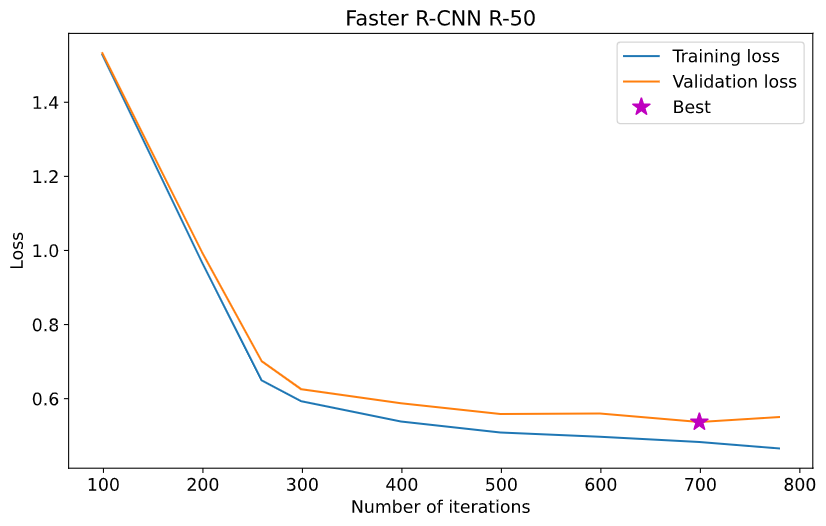
\includegraphics[width=\textwidth]{Sources/Figures/candies/Faster R-CNN R-50.png}
	\end{minipage}\hfill
	\begin{minipage}{0.5\textwidth}
		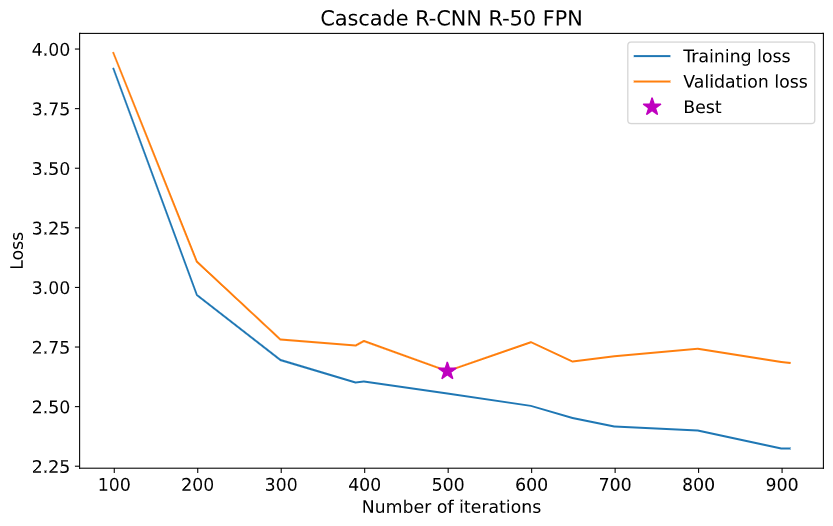
\includegraphics[width=\textwidth]{Sources/Figures/candies/Cascade R-CNN R-50 FPN.png}
	\end{minipage}\par
	\vskip\floatsep
	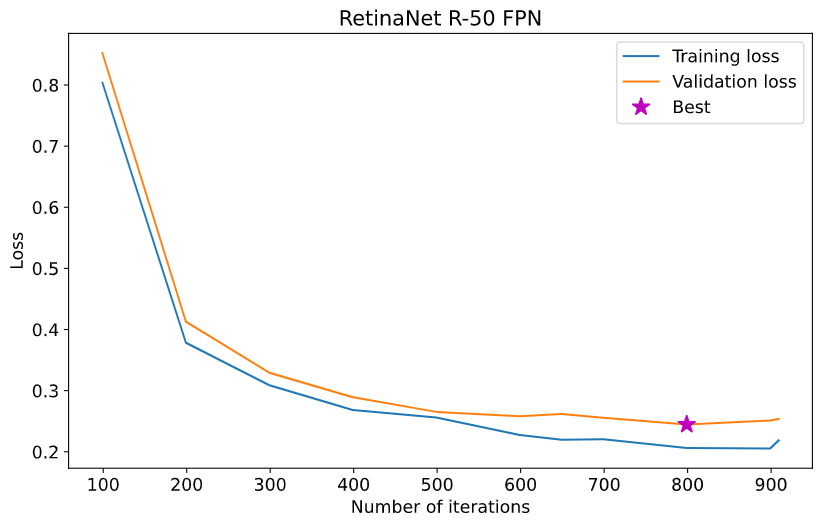
\includegraphics[width=0.5\textwidth]{Sources/Figures/candies/RetinaNet R-50 FPN.png}
	\caption{Loss curves of trained models on candies dataset.}
	\label{fig:candies_loss}
\end{figure}

\subsection*{Candies dataset}
The resulting AP metrics for the candies dataset can be seen in Table
\ref{tab:candies}. We can see that the AP is indeed higher than for the COCO
dataset (44.3 for Cascade R-CNN \cite{detectron}). Another observation we make
is that the main APs (AP, AP$_{50}$, AP$_{75}$) do not differ that much. And
in fact, they \bld{do not match with our hypothesis (b)} as the Cascade R-CNN is
the worst model. We strongly believe that this is caused by \bld{extremely small
	dataset size}. The test set consists only of 22 images. The random sample of
test images can thus greatly affect the resulting AP as the small sample may not
cover most of the cases of the images. Moreover the small training size also
\bld{causes overfitting} as we can see in the Figure \ref{fig:candies_loss}.

\begin{table}[H]
	\centering
	\begin{tabular}{l|c|c|c|c|c|c}
		Model                  & AP    & AP$_{50}$ & AP$_{75}$ & AP$_\text{large}$ & AP$_\text{medium}$ & AP$_\text{small}$ \\
		\hline
		RetinaNet R-50 FPN     & 66.09 & 99.27     & 77.98     & -                 & 66.12              & 30.00             \\
		Faster R-CNN R-50      & 65.99 & 98.98     & 78.49     & -                 & 66.00              & 60.00             \\
		Cascade R-CNN R-50 FPN & 65.24 & 97.93     & 77.13     & -                 & 65.27              & 25.00
	\end{tabular}
	\caption{AP for candies dataset. AP$_\text{large}$ could not be computed
		simply because there were not any larger bounding boxes.}
	\label{tab:candies}
\end{table}

Nevertheless, we can see that training a small dataset on our datasets can
produce relatively sufficient performance that can be used for additional
annotation of the datasets by using the models' predictions. The Figure
\ref{fig:candies_hard} shows an hard example of dense image with two false
positive predictions by RetinaNet model. In the top left corner of the image,
the model falsely detected a candy between two correctly detected candies. The
second false prediction is more interesting. The model predicted a candy out of
an area that actually looks like a candy to human eyes. But in fact, it is
the ends of two candy packagings that form the illusion.

\begin{figure}[H]

	\begin{subfigure}[t]{0.5\textwidth}
		\centering
		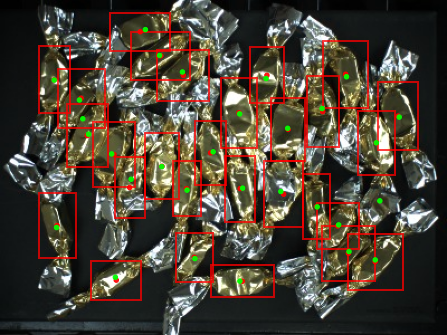
\includegraphics[width=\linewidth]{Sources/Figures/candies/actual_pred.png}
		\caption{The red rectangles are actual annotations. The green dots are
			the centers of the predictions. We do not include the rectangles for
			clarity as there are a lot of objects.}

	\end{subfigure}
	\begin{subfigure}[t]{0.5\textwidth}
		\centering
		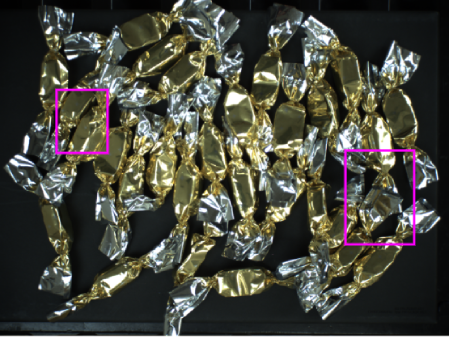
\includegraphics[width=\linewidth]{Sources/Figures/candies/false_positive.png}
		\caption{The false positive predictions.}

	\end{subfigure}

	\caption{Hard image predictions by RetinaNet.}
	\label{fig:candies_hard}
\end{figure}

The measured average inference times of each model is listed below in Table
\ref{tab:candies_time}. It was evaluated on Google Colab with NVIDIA Tesla T4
GPU and Intel Xeon CPU 2.20GHz. Each image had 300$\times$400px resolution. We
can see that RetinaNet is indeed the fastest of all models and all models meet
our hypothesis (d).


\begin{table}[H]
	\centering
	\begin{tabular}{l|c|c}
		Model                  & seconds per image & FPS                               \\
		\hline
		RetinaNet R-50 FPN     & 0.102             & \scriptsize $\sim$\normalsize9.80 \\
		Cascade R-CNN R-50 FPN & 0.167             & \scriptsize $\sim$\normalsize5.99 \\
		Faster R-CNN R-50      & 0.178             & \scriptsize $\sim$\normalsize5.62 \\
	\end{tabular}
	\caption{AP for candies dataset. AP$_\text{large}$ could not be computed
		simply because there were not any larger bounding boxes.}
	\label{tab:candies_time}
\end{table}

\begin{figure}[ht]
	\centering
	\begin{minipage}{0.5\textwidth}
		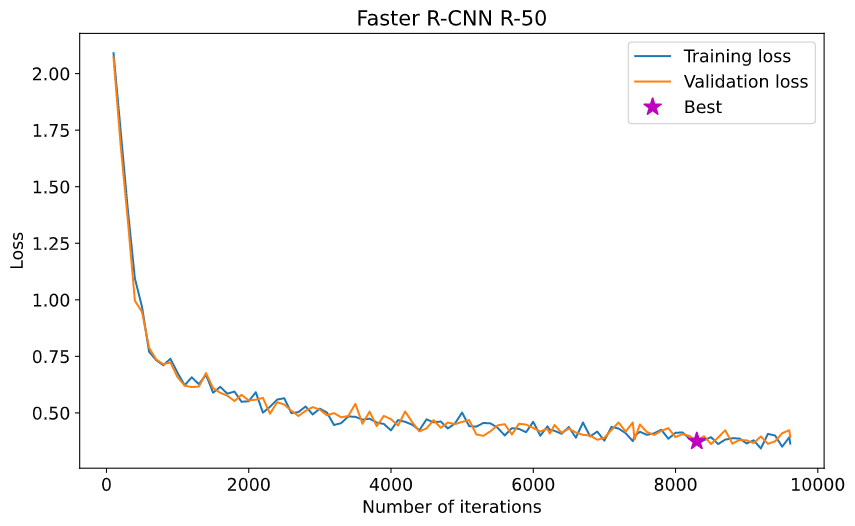
\includegraphics[width=\textwidth]{Sources/Figures/metal/metal_frcnn_loss.png}
	\end{minipage}\hfill
	\begin{minipage}{0.5\textwidth}
		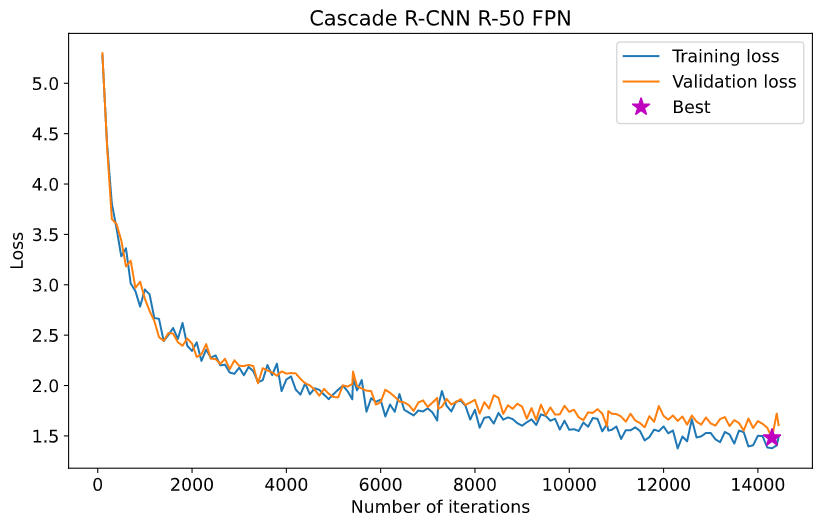
\includegraphics[width=\textwidth]{Sources/Figures/metal/metal_cascade_loss.png}
	\end{minipage}\par
	\vskip\floatsep
	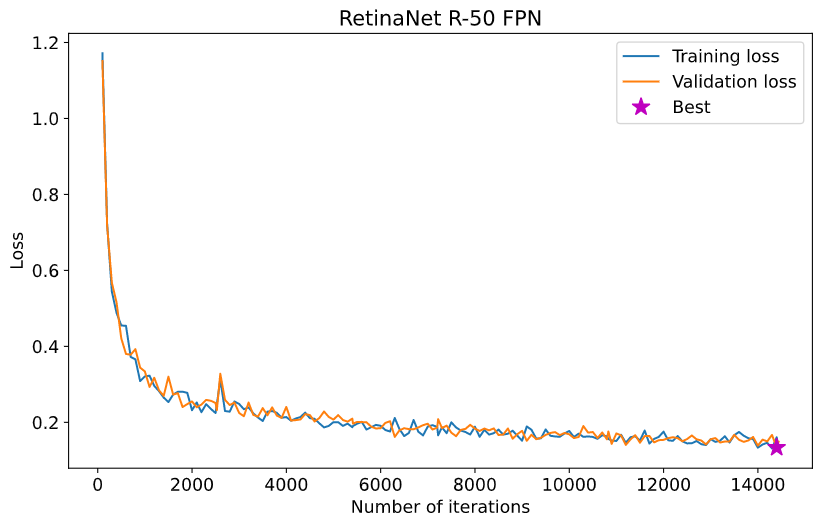
\includegraphics[width=0.5\textwidth]{Sources/Figures/metal/metal_retina_loss.png}
	\caption{Loss curves of trained models on metal parts dataset.}
	\label{fig:metal_loss}
\end{figure}

\subsection*{Metal parts dataset}
Since there are more classes in metal parts dataset, we visualize the metrics
as a heatmap in the Figure \ref{fig:metal_ap}. The loss curves are shown in
the Figure \ref{fig:metal_loss}. The results for this dataset correspond more to
the assumptions we have made in Section \ref{sec:hypotheses}. We believe this is
because of the larger size of the dataset. We can see that there is a
significant difference between the worst model Faster R-CNN and the best
performing model Cascade R-CNN (\small$\sim$\normalsize12 AP difference). The
main AP metric ratio between models is relatively similar among all classes
except the class 1, class 2, and class 4. RetinaNet can predict the first two
classes the best. We are not entirely sure of this behavior; however, the
objects of both classes are of greater sizes than the rest of the objects. This
could suggest that the RetinaNet can perform better on objects of
a bigger size.

\begin{figure}[H]
	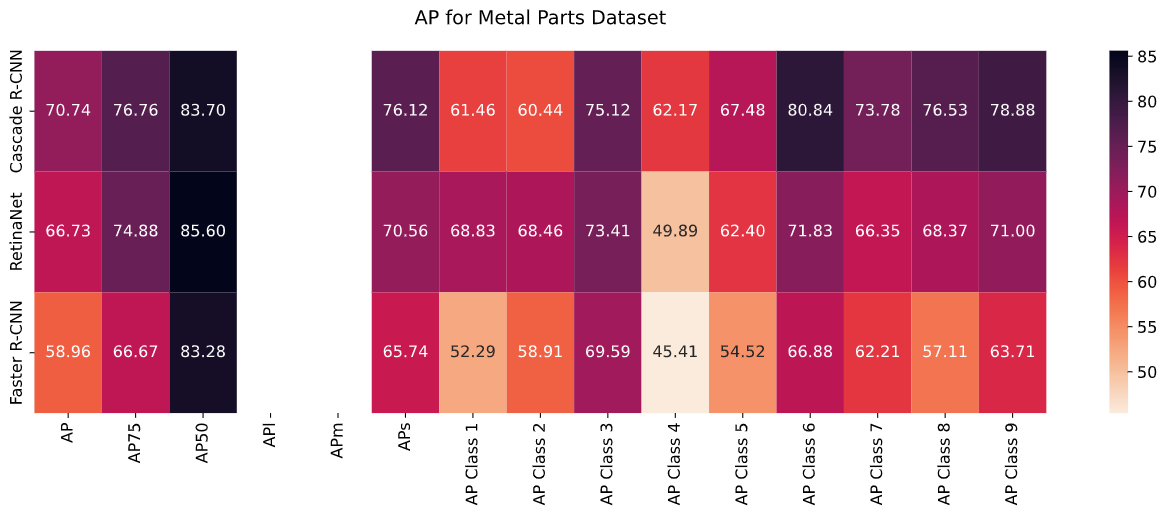
\includegraphics[width=\linewidth]{Sources/Figures/metal/metal_ap.png}
	\caption{AP table for metal parts dataset.}
	\label{fig:metal_ap}
\end{figure}

The hardest images for prediction were those with the class 4. The objects of
class 4 are relatively small. On top of that, they are very densely arranged in
the image (see Figure \ref{fig:metal_example} for illustration).

\begin{figure}[H]
	\centering
	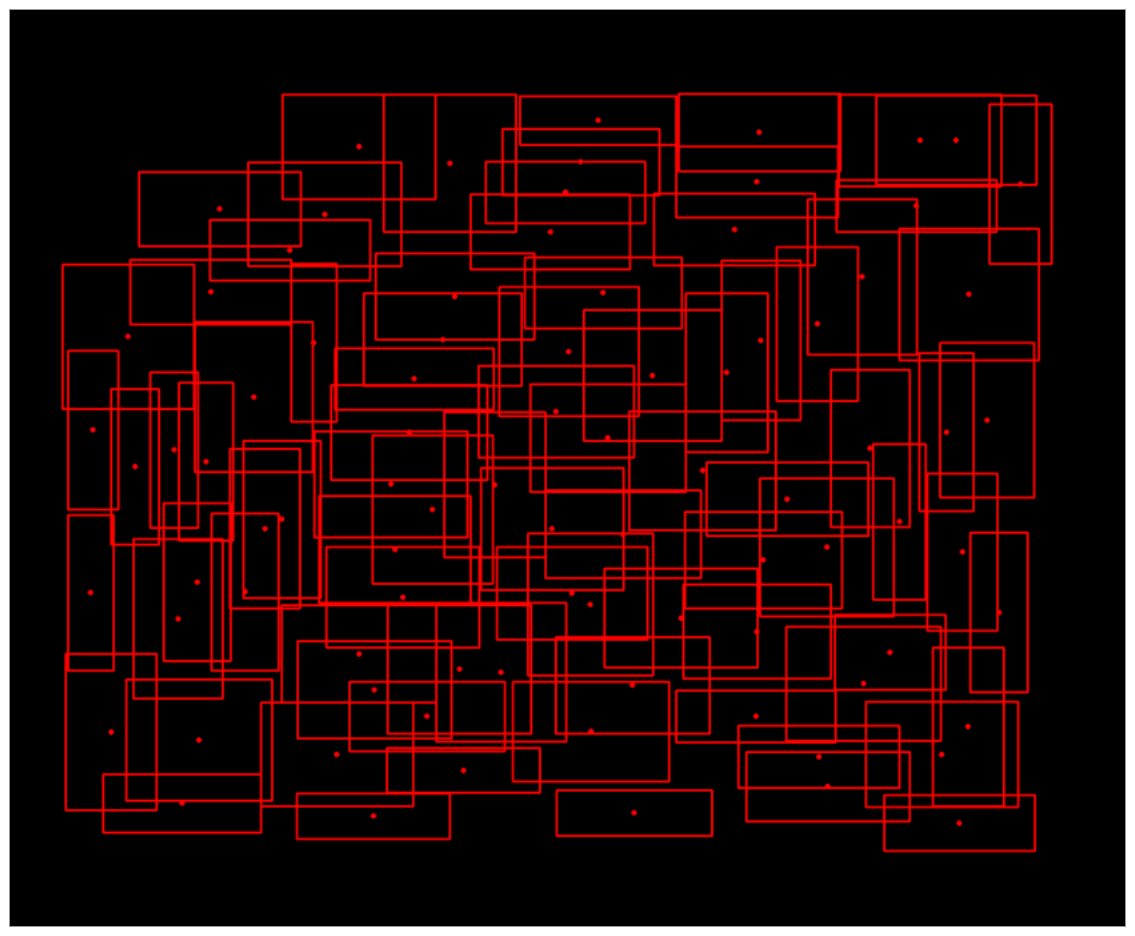
\includegraphics[width=0.45\textwidth]{Sources/Figures/metal/example.png}
	\caption{An illustration of density of metal parts dataset class 4
		objects.}
	\label{fig:metal_example}
\end{figure}

The measured inference times were greater than on candies dataset because of
larger image size (960$\times$800px). Evaluation was performed on the same
hardware specifications. The results are dipslayed in the Table
\ref{tab:metal_time}.

\begin{table}[H]
	\centering
	\small
	\begin{tabular}{l|c|c}
		Model                  & seconds per image & FPS                                \\
		\hline
		RetinaNet R-50 FPN     & 0.092             & \scriptsize $\sim$\normalsize10.87 \\
		Cascade R-CNN R-50 FPN & 0.180             & \scriptsize $\sim$\normalsize5.55  \\
		Faster R-CNN R-50      & 0.259             & \scriptsize $\sim$\normalsize3.86  \\
	\end{tabular}
	\normalsize
	\caption{AP for candies dataset. AP$_\text{large}$ could not be computed
		simply because there were not any larger bounding boxes.}
	\label{tab:metal_time}
\end{table}

\subsection*{Medical supplies dataset}
The resulting metrics visualized in the Figure \ref{fig:medical_ap} suggest that
we have overestimated the dataset's difficulty as we have achieved AP higher
than 80 for every model. Cascade R-CNN is indeed the best model but the
differences are not that big as in previous dataset. We suspect that the reason
behind the outstanding performance is that the very similar or even almost
identical images repeat in the dataset. This happens because the items in the
medical packages have prescribed locations and quantities. Therefore, the most
significant variance in the images is the arms of the human operator assembling
the packages. The most challenging class to predict was class 7.  The objects of
class 7 are white medical bandages (band-aids). The operator always places four
of those bandages in the package. Because the bandages are white, it is hard to
detect the correct quantity. The AP$_{\text{medium}}$ is low due to the same
problem. Most of the medium objects were the bandages.

\begin{figure}[H]
	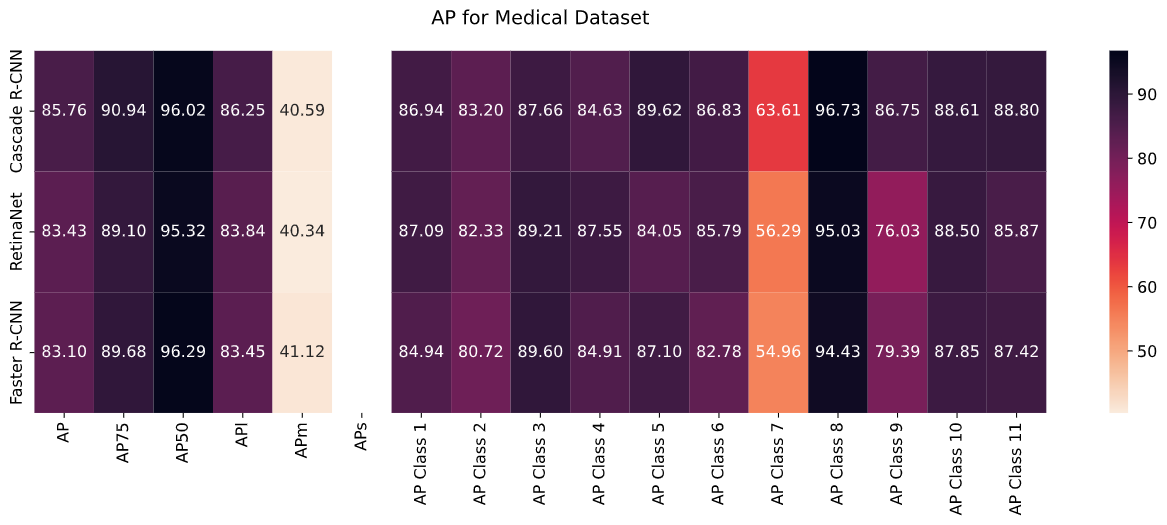
\includegraphics[width=\linewidth]{Sources/Figures/medical/medical_ap.png}
	\caption{AP table for medical supplies dataset.}
	\label{fig:medical_ap}
\end{figure}

Despite the exceptional results, the loss curves in Figure
\ref{fig:medical_loss} suggest an overfitting problem. We again believe that
the main reason of the issue is a relatively small dataset size. The medical
supplies dataset had the largest images by resolution (2464$\times$820px).
Therefore, the inference times were also the highest (see Table
\ref{tab:medical_times}); however, still achieve at least 2 FPS.

\begin{table}[H]
	\centering
	\begin{tabular}{l|c|c}
		Model                  & seconds per image & FPS                               \\
		\hline
		RetinaNet R-50 FPN     & 0.104             & \scriptsize $\sim$\normalsize9.61 \\
		Cascade R-CNN R-50 FPN & 0.202             & \scriptsize $\sim$\normalsize4.95 \\
		Faster R-CNN R-50      & 0.288             & \scriptsize $\sim$\normalsize3.47 \\
	\end{tabular}
	\caption{AP for candies dataset. AP$_\text{large}$ could not be computed
		simply because there were not any larger bounding boxes.}
	\label{tab:medical_times}
\end{table}

\begin{figure}[ht]
	\centering
	\begin{minipage}{0.5\textwidth}
		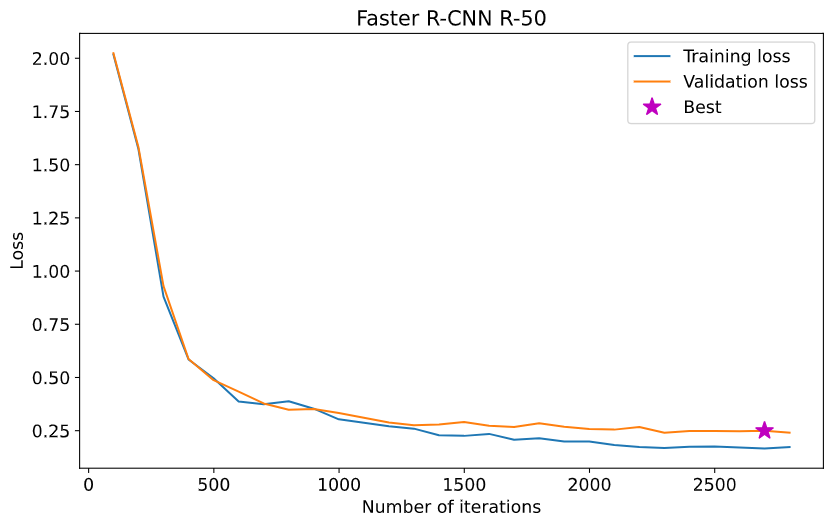
\includegraphics[width=\textwidth]{Sources/Figures/medical/frcnn_losses.png}
	\end{minipage}\hfill
	\begin{minipage}{0.5\textwidth}
		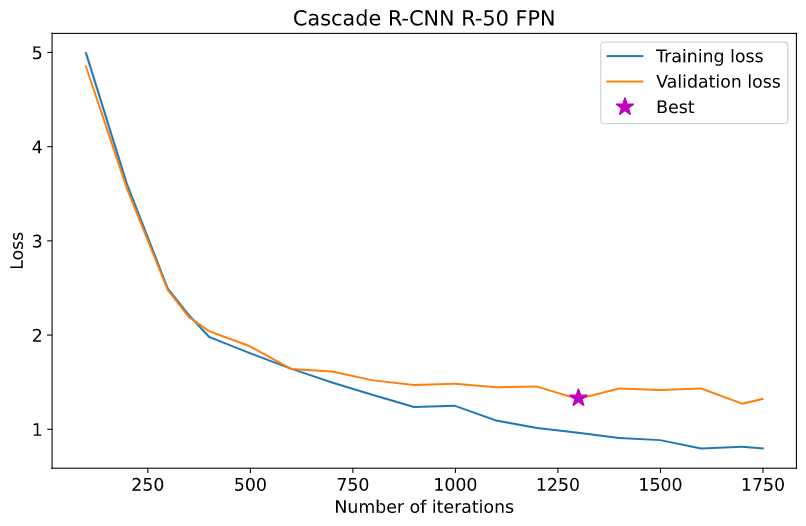
\includegraphics[width=\textwidth]{Sources/Figures/medical/cascade_losses.png}
	\end{minipage}\par
	\vskip\floatsep
	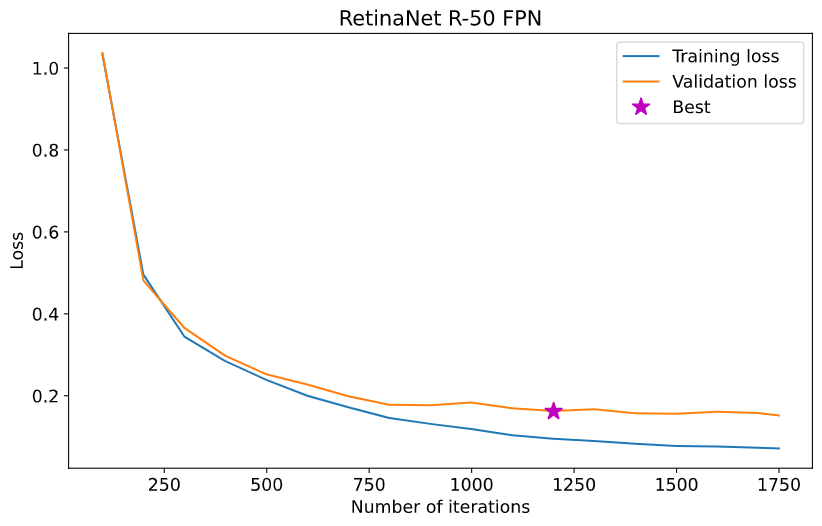
\includegraphics[width=0.5\textwidth]{Sources/Figures/medical/retina_losses.png}
	\caption{Loss curves of trained models on medical dataset.}
	\label{fig:medical_loss}
\end{figure}



\subsection*{Summary}
We would like to point out and wrap up the main observations of our evaluation
results in a few points below:
\begin{itemize}
	\item All models on all datasets overcame the COCO dataset AP (around 44 AP
	      for Cascade R-CNN).
	\item It is known that the bigger datasets produce better and more robust
	      models; however, a small dataset size such as in the case of candies dataset
	      can produce a sufficient model, e.g., for semi-automatic annotation uses
	      (the model predicts the bounding boxes and human annotator examines the
	      results and, if necessary, adjust the boundaries).
	\item The inference speed of RetinaNet is indeed the fastest. The
	      trade-off between AP and the speed is not that significant. RetinaNet
	      is about two times faster than Cascade R-CNN while achieving similar
	      AP. All models achieve the minimal speed of 2 FPS and can be used
	      for a real application. However, RetinaNet seems to be a viable
	      choice for more use cases.
	\item Models still struggle with images with high density of objects.
	      However, we believe that much larger dataset size and careful
	      fine-tuning of models could achieve decent results.
\end{itemize}




